\documentclass[tikz,border=6pt]{standalone}
\usepackage{tikz}
\usetikzlibrary{arrows.meta,calc,positioning,shapes.geometric}

\begin{document}
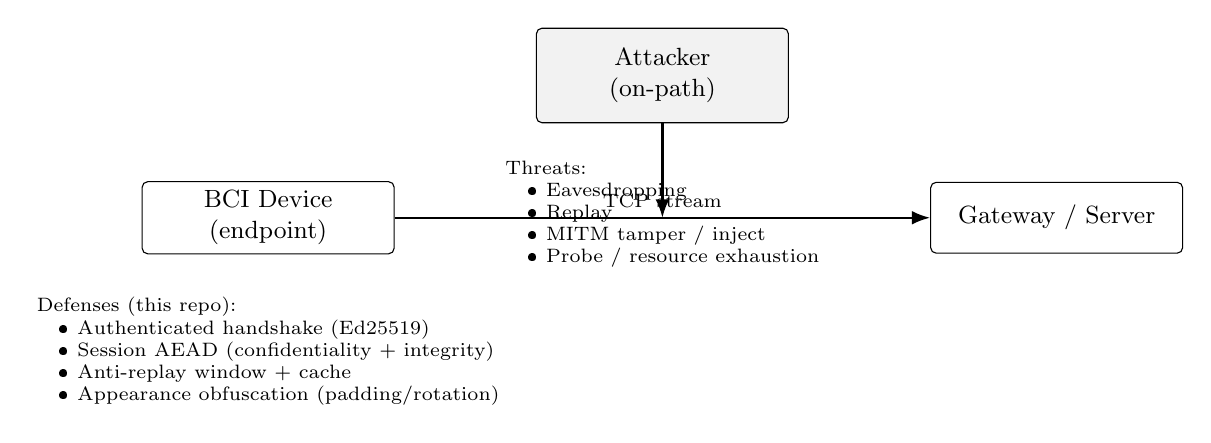
\begin{tikzpicture}[
  font=\small,
  nodebox/.style={draw,rounded corners=2pt,minimum width=3.2cm,minimum height=0.9cm,align=center},
  attacker/.style={draw,rounded corners=2pt,fill=gray!10,minimum width=3.2cm,minimum height=1.2cm,align=center},
  msg/.style={-Latex,thick},
  bullet/.style={font=\scriptsize,align=left},
]
  \node[nodebox] (dev) {BCI Device\\(endpoint)};
  \node[nodebox,right=6.8cm of dev] (srv) {Gateway / Server};
  \node[attacker,above=1.2cm of $(dev)!0.5!(srv)$] (atk) {Attacker\\(on-path)};

  \draw[msg] (dev) -- node[above,font=\scriptsize]{TCP stream} (srv);
  \draw[msg] (atk) -- ($(dev)!0.5!(srv)$);

  \node[bullet,below=10pt of atk] {
    Threats:\\
    \quad • Eavesdropping\\
    \quad • Replay\\
    \quad • MITM tamper / inject\\
    \quad • Probe / resource exhaustion
  };

  \node[bullet,below=12pt of dev] {
    Defenses (this repo):\\
    \quad • Authenticated handshake (Ed25519)\\
    \quad • Session AEAD (confidentiality + integrity)\\
    \quad • Anti-replay window + cache\\
    \quad • Appearance obfuscation (padding/rotation)
  };
\end{tikzpicture}
\end{document}
